\Def Кнезеровский граф $-$ G(n, k, 0), также обозначается $KG_{n, k}$, т. е. если $R_n=\overline{1..n}$, то $V=\{ S | S \subseteq R_n\!\! \wedge\!\! |S| = k \}$ и $E=\{ (A, B) | A \in V\!\! \wedge\!\! B \in V\!\! \wedge\!\! A\! \cap\! B = \varnothing \}$.

\underline{Оценка сверху с помощью клик}: Что такое клика в графе $KG_{n,k}$? Это, по сути, любой набор попарно непересекающихся k-элементных подмножеств множества $R_n$. Естественно, типичная клика выглядит так, как показано на рисунке. И её размер заведомо непревышает $\left[ \frac{n}{k} \right]$. В итоге получаем неравенство $\chi(KG_{n, k}) \geqslant \omega(KG_{n, k}) = \left[\frac{n}{k} \right]$. Интересный случай при $k=\left[ \frac{n}{3} \right] + 1$. Тогда $\omega(KG_{n, k}) = \left[ \frac{n}{k} \right] < 3$, т. е. в графе нет даже треугольников. Тем не менее, по теореме Ловаса хроматическое число $\geqslant \frac{n}{3}$. То есть, мы можем получить граф без треугольников со сколь угодно большим хром. числом.

\begin{center}
    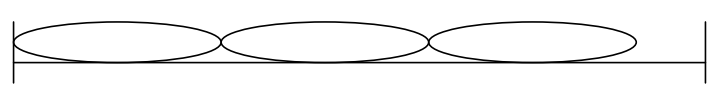
\includegraphics[scale=0.4]{images/Knezer_clique.png}
\end{center}

\underline{Оценка снизу с помощью независимых множеств}: По теореме Эрдёша-Ко-Радо \newline
$\alpha(KG_{n, k})=C^{k-1}_{n-1}$(если не разрешат использовать её, то возьмём все множества, пересекающиеся по 1, тогда получим $\alpha(KG_{n, k}) \geqslant C^{k-1}_{n-1}$), значит, по нашей оценке 
$$\chi(KG_{n, k}) \geqslant \frac{C^k_n}{C^{k-1}_{n-1}} = \frac{n}{k}$$ \\
Стоит заметить, что эта оценка почти не отличается от предыдущей, только на 1 хуже, если n не делится на k.

\underline{Простые верхние оценки}: Самая простая оценка: n. Поочерёдно будем брать множества, пересекающие по i для $i \in R_n$. Тогда каждый элемент i-го множества можно покрасить в один и тот же цвет, так как между ними нет рёбер, а всего множеств n. Эту оценку можно немного улучшить: Красим так же, как и раньше до n-k+1. Тогда неиспользованных чисел остаётся только k-1<1 для любой непокрашенной вершины, значит, это меньше, чем полноценная вершина, значит, непокрашенных вершин не осталось. Улучшенная оценка: $\chi(KG_{n, k}) \leqslant n-k+1$.

\underline{Лучшая оценка}: Повторим раскарску, но теперь до n-2k+1. Тогда все оставшиеся веришны - подмножества $R_n \setminus R_{n-2k+1}$. Тогда чисел остаётся всего 2k-1, и значит, любые две веришны пересекаются, значит, можем покрасить их в ещё один цвет и $\chi(KG_{n, k}) \leqslant n-2k+2$.

\underline{Примеры}: \\
$-$ $KG_{n, 1}=K_n$ \\
$-$ $KG_{n, k}=(V, \varnothing)$, если $k > \frac{n}{2}$ \\ 
$-$ $KG_{n, \frac{n}{2}}$ $-$ паросочетание \\
$-$ $KG_{5, 2}$ $-$ граф Петерсена
